\documentclass[12pt]{article}

\usepackage{amsmath}
\usepackage[authoryear,round]{natbib}
\usepackage{hyperref}



\textwidth=6.2in
\textheight=8.5in
\oddsidemargin=.1in
\evensidemargin=.1in
\headheight=-.3in

\newcommand{\scscst}{\scriptscriptstyle}
\newcommand{\scst}{\scriptstyle}
\newcommand{\Rfunction}[1]{{\texttt{#1()}}}
\newcommand{\Rmethod}[1]{{\texttt{#1}}}  
\newcommand{\Rclass}[1]{{\texttt{#1}}}
\newcommand{\Robject}[1]{{\texttt{#1}}}
\newcommand{\Rpackage}[1]{{\textit{#1}}}
\newcommand{\code}[1]{{\texttt{#1}}}
\bibliographystyle{plainnat}

\title{Outline: Analysis of High Throughput Flow Cytometry Data using \Rpackage{plateCore}}

%%%%%%%%%%%%%%%%%%%%%%%%%%%%%%%%%%%%%%%%%%%%%%%%%%%%%%%%%%%%%%%%%%%%%%%%%%%
\usepackage{Sweave}
\begin{document}
\maketitle

\clearpage
%%%%%%%%%%%%%%%%%%%%%%%%%%%%%%%%%%%%%%%%%%%%%%%%%%%%%%%%%%%%%%%%%%%%%%%%%%%%%%%%%%%%%%%%%%%%%%%%%%%%%%%%%%%%%%%%%%%%%%%%%%%%%%%%%%%
\section*{Abstract}
\subsection*{Background}
High throughput flow studies are often run in a 96 or 384-well plate format, with a number of different samples, 
controls, and antibodies-dye conjugates present on the plate. Analyzing the output from the cytometer requires keeping track ofthe contents
of each well, matching sample wells with control wells, gating each well/channel separately, making the appropriate plots, assessing quality, and
summarizing the results. This can be a monumental task using traditional point-and-click software packages, even when multiple instances are
deployed. We developed \Rpackage{plateCore} as an R/Bioconductor packaged to make processing and analysis of large, complex flow cytometry (FCM) datasets
easier. 

\subsection*{Methods}
\Rpackage{plateCore} was used to analyze the results from a BD FACS\texttrademark CAP screening experiment where 5 PBMC samples 
were assayed for 189 different human cell surface markers. 
This same dataset was also analyzed by a cytometry expert using FlowJo\texttrademark.

\subsection*{Results}
Positive markers identified using \Rpackage{plateCore} are in good agreement with those found using FlowJo\texttrademark analysis.

\subsection*{Conclusions}
\Rpackage{plateCore} provides a reproducible, objective platform for analyzing high throughput flow experiments. The R/Bioconductor 
implementation allows bioinformaticians and statisticians access to the data, which should further the development of automated
analysis methods.

\clearpage
%%%%%%%%%%%%%%%%%%%%%%%%%%%%%%%%%%%%%%%%%%%%%%%%%%%%%%%%%%%%%%%%%%%%%%%%%%%%%%%%%%%%%%%%%%%%%%%%%%%%%%%%%%%%%%%%%%%%%%%%%%%%%%%%%%
\section*{Introduction}
Analysis of flow cytometry high content screening (FC-HCS) experiments requires a systematic approach to
preprocessing, gating (i.e., filtering), and summarizing large amounts of data. Ideally these steps would be automated,
allowing analysis pipelines to be robust, objective, and match the high-throughput capacity of modern cytometers. 
Unfortunately, current approaches to FC-HCS analysis methods are semi-automated at best,
often requiring significant manual intervention to identify cells of interest and set the appropriate gates. 
Since the manual contribution is subjective and prone to error when working with large numbers of samples (ref Holden?), it
is desirable to develop programmatic approaches to process the data.

Flow cytometry packages available through the Bioconductor (ref) project provide an open analysis platform that
can be used by cytometrists, bioinformaticians, and statisticians to develop new analysis approaches that
enable automated processing. The \Rpackage{flowCore} (ref) package contains the framework for importing, transforming, gating, and
organizing raw flow cytometry data. \Rpackage{flowViz} (ref) supports sophisticated visualizations based on Trellis (ref?) displays. 
\Rpackage{flowClust} (ref) implements model-based clustering approaches for automated gating. \Rpackage{plateCore}
extends the \Rpackage{flowCore} and \Rpackage{flowViz} packages to work on \Robject{flowPlate} objects that represent
large flow datasets. The combination of these packages provides a set of freely available, flexible, and computationally efficient FC-HCS tools. 

An example of the progression from raw FCM data files to a completed \Rpackage{plateCore} analysis is shown in Figure~\ref{fig:analysis}.
List mode FCS files for a single plate are read into a \Robject{flowSet} using \Rpackage{flowCore}, and then a \Robject{flowPlate} is created by integrating
the plate annotation file with the \Robject{flowSet}. The \Robject{flowPlate} is then compensated, data quality is assessed, and gates
are set according to a negative control. These control gates are then applied to test wells to find cells that have specific staining
in channels of interest. Assuming that the automated gates do not require adjustment, and that there are no missing wells or other major problems,
the analysis of a single plate can be accomplished in 10-12 lines of code. While this same analysis can be performed relatively quickly in 
other flow cytometry software packages, it can be difficult to reproduce the gating decisions made by a single expert user.

In addition to subjective gating, the lack of a standard format for describing large flow experiments also
makes it difficult for anyone other than the original experimenter to replicate an analysis. 
The adoption of ACS specifications (ref) should make it easier to access metadata in future flow studies, but currently
this information is typically provided as a pictorial layout of a 96 well plate. 
Since the creation of \Robject{flowPlate} requires users to make a defined sample annotation file, plate layouts
can then be easily shared along with the raw FCS2.0/3.0 files. Also, this annotation can then be accessed
when working with \Robject{flowPlates} using either \Rpackage{flowCore} or \Rpackage{flowViz} functions.
The standard format for \Rpackage{plateCore} sample annotations provides a convenient way to manage the plate metadata
associated with complex FC-HCS experiments.

\Rpackage{plateCore} is not designed to be a GUI driven end-user tool, but rather to help develop a standardized platform for the analysis of FC-HCS data.
These analyses often represent a collaborative effort between cytometry experts who generate the data and the quantitative individuals who help
deal with the large volume information. In order for this collaboration to work, the cytometrists must have confidence in the
results of the automated analysis. To this point, we demonstrate the equality of our results to those produced by an expert
cytometrist using FlowJo\texttrademark.

%Since the layout of FC-HCS plates often changes from experiment
%to experiment, the annotation for each well needs to be customized for each
%\Rclass{flowPlate}. \Rpackage{plateCore} uses an approach that is very similar to the cell-based high throughput screening \Rpackage{cellHTS2} package (ref),
%where users must provide a \textit{plate configuration} file for each dataset. Once the cell level data has
%been analyzed in \Rpackage{plateCore}, the summary well information (i.e., percentage of positive cells and median
%signal intensities) can be imported into tools like \Rpackage{cellHTS2}, since FC-HCS experiments are just one 
%type of cell-based high throughput screens.

\begin{figure}
\centering
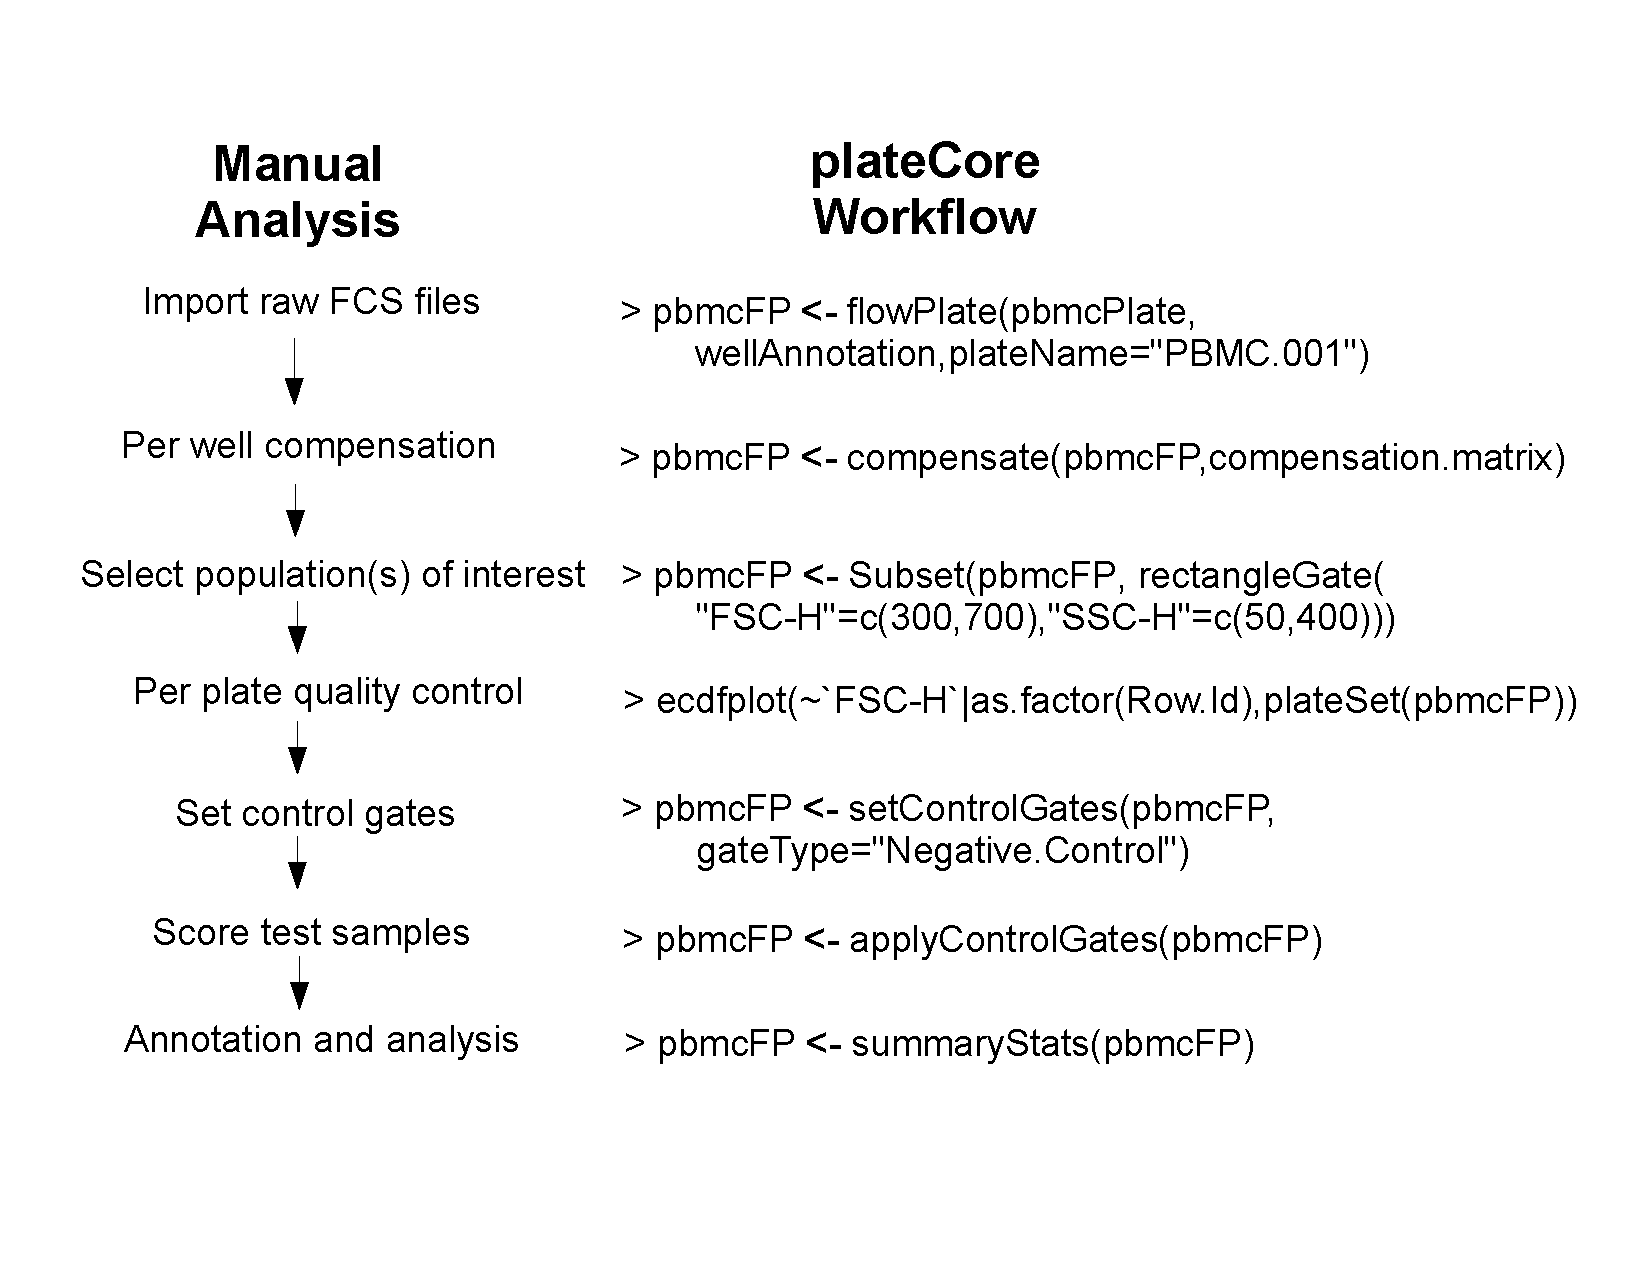
\includegraphics[width=7in,height=6in]{analysisSteps.pdf}
\caption{Typical plateCore workflow on the left, and examples of each step from a sample analysis are shown on the right.
Generating reports and plots is a multi-step that typically involves merging output from several plates, and the required
code is not shown here.
If necessary, the threshold control gates created automatically from \Rfunction{setControlGates} are adjusted based on input from flow experts. 
These new gates are established based on the gap between negative and positive test samples, whereas the automated
control gates were set using only negative control wells.}
\label{fig:analysis}
\end{figure}
 
%%%%%%%%%%%%%%%%%%%%%%%%%%%%%%%%%%%%%%%%%%%%%%%%%%%%%%%%%%%%%%%%%%%%%%%%%%%%%%%%%%%%%%%%%%%%%%%%%%%%%%%%%%%%%%%%%%%%%%%%%%%%%%%%%%%
\clearpage
\section*{Materials and Methods}
\subsection*{Data}

The peripheral blood mononucleocyte (PBMC) data used in this study consists of 5 samples that were analyzed on 96-well plates
using BD FACS\texttrademark CAP (ref). On each plate, there are 189 different human cell surface antibody-dye conjugates that
are arrayed 3 per well (63 test wells), along with 30 isotype control wells and 3 unstained controls.
Test antibodies and isotypes are arrayed 3 per well, and the data was compensated
on the cytometer (BD FACSCalibur\texttrademark). The 189 antibodies were selected to provide a broad expression profile
for a large number of cell surface markers, including 103 proteins with GO annotation for receptor activity, 80
for immune response, and 55 for signal transduction. The raw data is available for download from http://www.ficcs.org as
"plateData.tar.gz" file. The plate configuration is also included in the archive as \textit{maskPlateDesc.csv}, although
the antibody names have been masked. (Note: I need to update the description so it's compatible with the latest version of plateCore).

%%%%%%%%%%%%%%%%%%%%%%%%%%%%%%%%%%%%%%%%%%%%%%%%%%%%%%%%%%%%%%%%%%%%%%%%%%%%%%%%%%%%%%%%%%%%%%%%%%%%%%%%%%%%%%%%%%%%%%%%%%%%%%%%%%%
\subsection*{Analysis}

The goal of the PBMC FACS\texttrademark CAP study was to look for positive staining for the 189 different cell
surface markers in lymphocytes. The \Rpackage{plateCore} scripts used to perform the analysis are provided 
in supplementary materials. Briefly, the FCM files are first processed using a combination of static (\Robject{rectangleGate})
and data driven (\Robject{norm2filter}) gates to pick out the lymphocytes in the forward (FSC) and side scatter (SSC)
channels.  The quality of the data was then assessed by looking for fluidic events such as bubbles,
pressure drops, or large aggregates that can shift the baseline fluorescence readings. 
Fluidic events can often be identified by plotting the emprical cumulative density (ecdf) plots of FSC
values for each well, and looking for distributions shifted relative to other wells (ref Nolwenn's paper). Based on the ecdf
plots, several wells were further investigated by cytometry experts who determined that the shifts were in an acceptable range.
Next the threshold between positive and negative cells are determined using the isoytpe controls, which provide a gross estimate
of non-specific binding in the primary antibodies. One-dimensional gates are created using using the isotype thresholds, and these
gates are applied to identify cells that are positively stained for each marker. 

%%%%%%%%%%%%%%%%%%%%%%%%%%%%%%%%%%%%%%%%%%%%%%%%%%%%%%%%%%%%%%%%%%%%%%%%%%%%%%%%%%%%%%%%%%%%%%%%%%%%%%%%%%%%%%%%%%%%%%%%%%%%%%%%%%%
\clearpage
\section*{Results}
\subsection*{\Rpackage{plateCore} Output}

The output for the analysis of each plate was stored in a \Robject{flowPlate}, a data structure which contains the raw
FCM input along with isotype gating results. The \Robject{wellAnnotation} for each \Robject{flowPlate} was then merged
into a single \Robject{data.frame}, containing the percent positive results from each plate. These values can then visualized
using microarray tools in R (Figure~\ref{fig:pbmcHeat}). 

Once a marker of interest has been identified, the next step is usually to make density or dotplots of the signals from each
plate. Although these plots can be created individually, it is more convenient to have a combined data object so that results 
from multiple \Robject{flowPlates} can be quickly summarized. \Rpackage{plateCore} supports combining \Robject{flowPlates} using
the \Rfunction{fpbind} function. 
\begin{Schunk}
\begin{Sinput}
> virtPlate <- fpbind(plate1,plate2,plate3,plate4,plate5)
\end{Sinput}
\end{Schunk}
This virtual plate can then be used to make histograms for particular markers, such as CDbd69 which showed variable levels of
expression between the different donors (Figure~\ref{fig:pbmcCDbd69}). 
\begin{Schunk}
\begin{Sinput}
> densityplot(~ `FL2-H` | as.factor(plateName),
+ 	virtPlate,filterResult="Negative.Control")
\end{Sinput}
\end{Schunk}

\begin{figure}
\centering
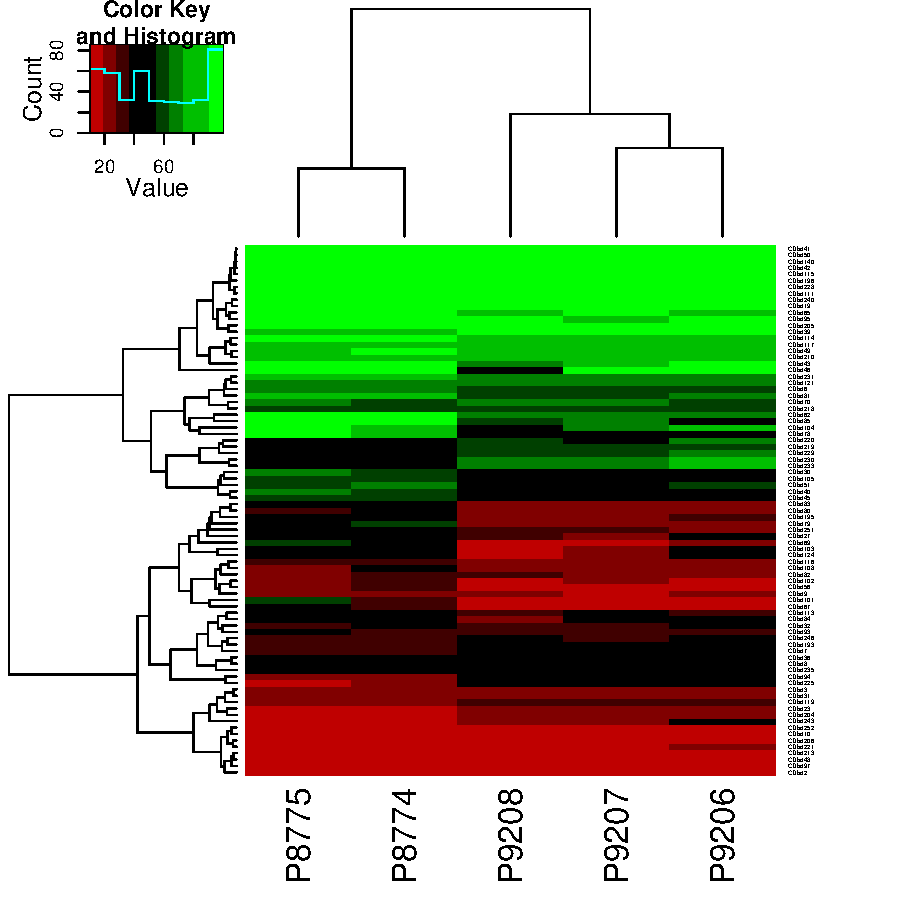
\includegraphics{outline-pbmcHeat}
\caption{Heatmap showing the percentage of positive cells from the 5 different PBMC lymphocyte plates. Only the 83 markers
that had $\ge$ 10\% positive cells are shown here.}
\label{fig:pbmcHeat}
\end{figure}

\begin{figure}
\centering
\begin{Schunk}
\begin{Soutput}
Scalable Robust Estimators with High Breakdown Point (version 0.4-07)
\end{Soutput}
\end{Schunk}
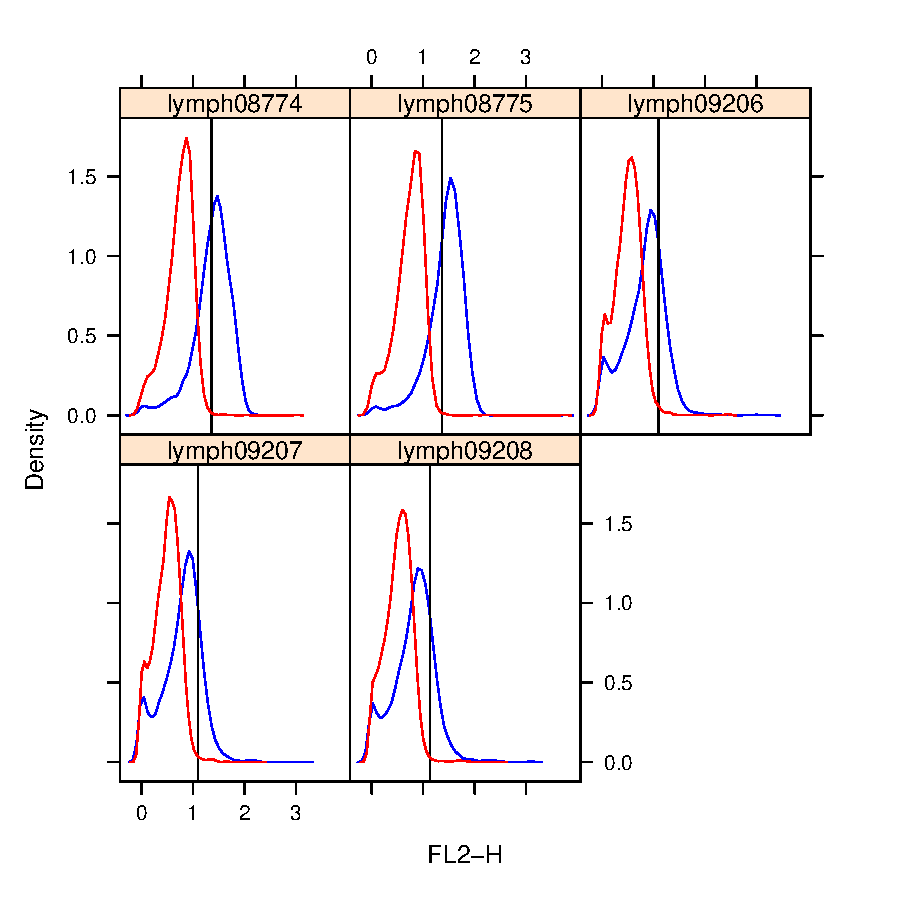
\includegraphics{outline-pbmcCDbd69}
\caption{Dotplots for CDbd69, which is differentially expressed between the 5 PBMC plates. Isotypes are shown in green and
test wells are in magenta.}
\label{fig:pbmcCDbd69}
\end{figure}

%%%%%%%%%%%%%%%%%%%%%%%%%%%%%%%%%%%%%%%%%%%%%%%%%%%%%%%%%%%%%%%%%%%%%%%%%%%%%%%%%%%%%%%%%%%%%%%%%%%%%%%%%%%%%%%%%%%%%%%%%%%%%%%%%%%
\clearpage
\subsection*{Comparison to Manual Analysis}

The 5 pmbc plates were also analyzed using FlowJo$^{\text{TM}}$, which is one of the standard FCM data analysis platforms.
BD FACS$^{\text{TM}}$ CAP is designed as a screening tool to help identify markers for additional analysis. Since it is 
not practical to have controls specific to each of the 189 antibody-dye conjugates, isotypes were chosen according to the
most common antibody subtypes. Cytometry experts initially set gates according to the isotype controls, and then move the
gates based on positive and negative test samples. Figure~\ref{fig:pcVSman} shows how the results from FlowJo$^{\text{TM}}$ compare to \Rpackage{plateCore}.

\begin{figure}
\centering
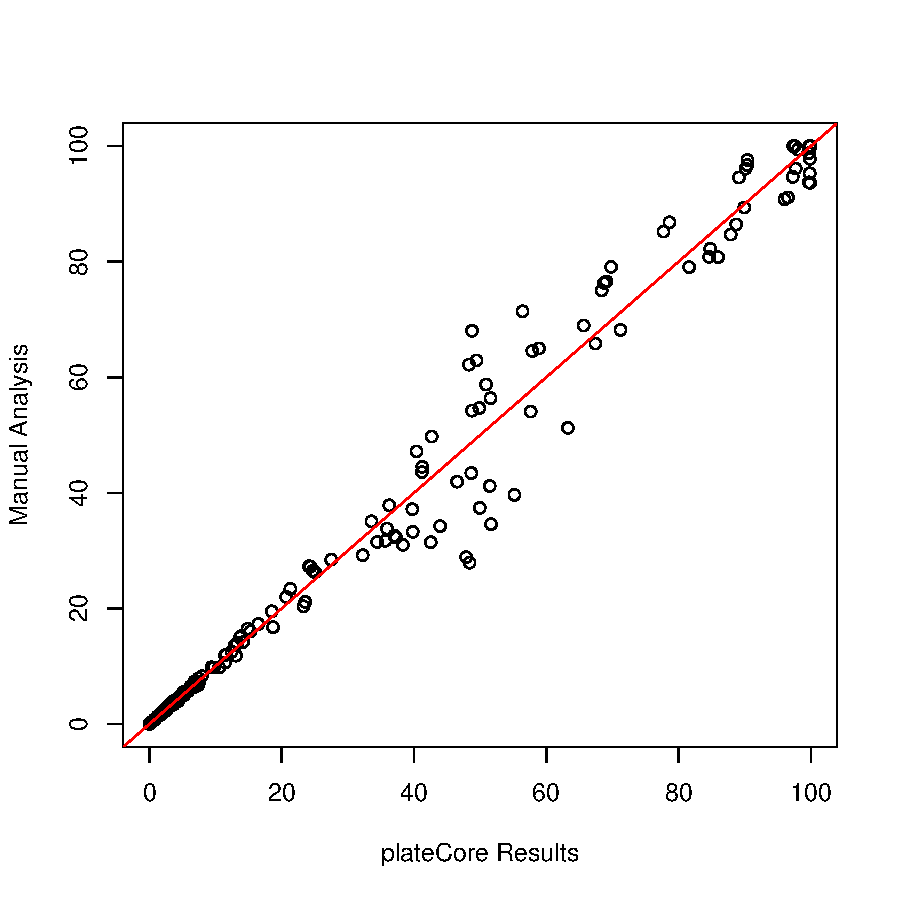
\includegraphics{outline-pcVSman}
\caption{Percent positive results for 189 markers analyzed using either \Rpackage{plateCore} or manually using FlowJo$^{\text{TM}}$. (Note: Need to get real
data in this plot)}
\label{fig:pcVSman}
\end{figure}

%%%%%%%%%%%%%%%%%%%%%%%%%%%%%%%%%%%%%%%%%%%%%%%%%%%%%%%%%%%%%%%%%%%%%%%%%%%%%%%%%%%%%%%%%%%%%%%%%%%%%%%%%%%%%%%%%%%%%%%%%%%%%%%%%%%
\clearpage
\section*{Discussion}

The PBMC example shows that a complex analysis of a 96-well plate, stained with 189 antibodies,
can be constructed in 15-20 lines of code using \Rpackage{plateCore}. Lymphocytes were selected
using \Rpackage{flowCore} gates and visualized using \Rpackage{flowViz} plots. One-dimensional 
gates were constructed using isotype wells and applied to the test wells to identify positive cells.

Given a \textit{plate configuration} file, this same approach can be used to analyze any
negative control based FC-HCS study. Although adjustments to the automatically generated negative control gates may be needed,
these changes change be incorporated into the analysis script and reproduced at a later time.

(Need some additional paragraphs about why plateCore is wonderful).

%%%%%%%%%%%%%%%%%%%%%%%%%%%%%%%%%%%%%%%%%%%%%%%%%%%%%%%%%%%%%%%%%%%%%%%%%%%%%%%%%%%%%%%%%%%%%%%%%%%%%%%%%%%%%%%%%%%%%%%%%%%%%%%%%%%
\section*{References/Recent Related Publications}
\begin{itemize}
\item flowCore manuscript in Cytometry A\\
Gives an overview of flowCore data structures, transformation and gating examples, quality control checks (flowQ), and 
flowCore analysis philosophy.\\
\item Using flowViz to Visualize Flow Cytometry Data, Bioinformatics\\
Uses flowViz to make xyplots, ecdfplots, and time plots of GvHD data. Makes the case that visualizations can be used to aid automation.
\item Quality Assessment of Ungated Flow Cytometry data in High Throughput experiments, Cytometry A, GvHD data\\
Visualizing data: xyplots, histograms, ecdfplots, boxplots, and contour plots.\\
Outlier detection (Grubbs and KS)\\
Using flowViz/Core graphical output for quality assessment\\
\item Analysis of flow cytometry data using an automatic processing tool, Cytometry Part A\\
Automated analysis in Matlab.\\
\end{itemize}


\end{document}
